%%%%%%%%%%%%%%%%%%%%%%%%%%%%%%%%%%%%%%%%%
% Beamer Presentation
% LaTeX Template
% Version 1.0 (10/11/12)
%
% This template has been downloaded from:
% http://www.LaTeXTemplates.com
%
% License:
% CC BY-NC-SA 3.0 (http://creativecommons.org/licenses/by-nc-sa/3.0/)
%
%%%%%%%%%%%%%%%%%%%%%%%%%%%%%%%%%%%%%%%%%

%----------------------------------------------------------------------------------------
%	PACKAGES AND THEMES
%----------------------------------------------------------------------------------------

\documentclass[10pt]{beamer}	

\mode<presentation> {

% The Beamer class comes with a number of default slide themes
% which change the colors and layouts of slides. Below this is a list
% of all the themes, uncomment each in turn to see what they look like.

%\usetheme{default}
%\usetheme{AnnArbor}
%\usetheme{Antibes}
%\usetheme{Bergen}
%\usetheme{Berkeley}
%\usetheme{Berlin}
%\usetheme{Boadilla}
%\usetheme{CambridgeUS}
%\usetheme{Copenhagen}
\usetheme{Darmstadt}
%\usetheme{Dresden}
%\usetheme{Frankfurt}
%\usetheme{Goettingen}
%\usetheme{Hannover}
%\usetheme{Ilmenau}
%\usetheme{JuanLesPins}
%\usetheme{Luebeck}
%\usetheme{Madrid}
%\usetheme{Malmoe}
%\usetheme{Marburg}
%\usetheme{Montpellier}
%\usetheme{PaloAlto}
%\usetheme{Pittsburgh}
%\usetheme{Rochester}
%\usetheme{Singapore}
%\usetheme{Szeged}
%\usetheme{Warsaw}

% As well as themes, the Beamer class has a number of color themes
% for any slide theme. Uncomment each of these in turn to see how it
% changes the colors of your current slide theme.

%\usecolortheme{albatross}
%\usecolortheme{beaver}
%\usecolortheme{beetle}
%\usecolortheme{crane}
%\usecolortheme{dolphin}
%\usecolortheme{dove}
%\usecolortheme{fly}
%\usecolortheme{lily}
%\usecolortheme{orchid}
%\usecolortheme{rose}
%\usecolortheme{seagull}
%\usecolortheme{seahorse}
%\usecolortheme{whale}
%\usecolortheme{wolverine}

%\setbeamertemplate{footline} % To remove the footer line in all slides uncomment this line
%\setbeamertemplate{footline}[page number] % To replace the footer line in all slides with a simple slide count uncomment this line
\setbeamertemplate{enumerate mini template}{\insertenumlabel}
\setbeamertemplate{navigation symbols}{} % To remove the navigation symbols from the bottom of all slides uncomment this line
\setbeamertemplate{caption}[numbered]
}
\graphicspath{{images/}}

%\usepackage{sansmathaccent}
%\pdfmapfile{+sansmathaccent.map}

\usepackage[utf8]{inputenc}
\usepackage[portuguese]{babel}
\usepackage{graphicx} % Allows including images
\usepackage{booktabs} % Allows the use of \toprule, \midrule and \bottomrule in tables
\usepackage{caption}
\usepackage{subcaption}
\usepackage{float}
\usepackage{multirow} 
\usepackage{bigstrut}
\usepackage{textcomp}
\usepackage{listings}
\usepackage{color}

%\usepackage{enumitem}


\definecolor{codegreen}{rgb}{0,0.6,0}
\definecolor{codegray}{rgb}{0.5,0.5,0.5}
\definecolor{codepurple}{rgb}{0.58,0,0.82}
\definecolor{backcolour}{rgb}{0.95,0.95,0.92}

\lstdefinestyle{mystyle}{
	backgroundcolor=\color{backcolour},   
	commentstyle=\color{codegreen},
	keywordstyle=\color{magenta},
	numberstyle=\tiny\color{codegray},
	stringstyle=\color{codepurple},
	basicstyle=\tiny,
	breakatwhitespace=false,         
	breaklines=true,                 
	captionpos=b,                    
	keepspaces=true,                 
	numbers=left,                    
	numbersep=5pt,                  
	showspaces=false,                
	showstringspaces=false,
	showtabs=false,                  
	tabsize=2
}

\lstset{style=mystyle}

%----------------------------------------------------------------------------------------
%	TITLE PAGE
%----------------------------------------------------------------------------------------

\title{Arquitetura orientada a servi\c{c}os baseada no RAMI4.0 para o compartilhamento da mem\'{o}ria digital do produto ao longo da cadeia de suprimentos} % The short title appears at the bottom of every slide, the full title is only on the title page

\author{Henrique Abrantes Vitoi} % Your name

\institute[Poli-USP] % Your institution as it will appear on the bottom of every slide, may be shorthand to save space
{
	 % Your institution for the title page
Escola Politécnica da Universidade de São Paulo \\
Engenharia de Controle e Automação Mecânica

%\medskip
%\textit{hvitoi@usp.br} % Your email address
}
\date{\today} % Date, can be changed to a custom date

\begin{document}
	
%----------------------------------------------------------------------------------------
%	PRESENTATION SLIDES
%----------------------------------------------------------------------------------------

\begin{frame}
	\titlepage % Print the title page as the first slide
\end{frame}

\begin{frame}
	\frametitle{Sumário} % Table of contents slide, comment this block out to remove it
	\tableofcontents % Throughout your presentation, if you choose to use \section{} and \subsection{} commands, these will automatically be printed on this slide as an overview of your presentation
\end{frame}

%------------------------------------------------
\section{Introdução}
%------------------------------------------------

\begin{frame}
	\frametitle{Informações}
	
	\begin{itemize}
		\item Autor: Henrique Abrantes Vitoi
		\item Orientação: Prof. Dr. Fabrício Junqueira
		\item Coorientação: Prof. Dr. Paulo Eigi Miyagi
		\item Departamento de Engenharia Mecatrônica e de Sistemas Mecânicos
		
	\end{itemize}

\end{frame}
%---
\begin{frame}
	\frametitle{Contextualização}
		
	\begin{itemize}
		\item Cenário intrinsecamente globalizado
		\item Necessidade de eficiência em troca de informações, serviços e mercadoria
		\item Eficiência logística
		\item Logística da informação
	\end{itemize}

\end{frame}
%---
\begin{frame}
	\frametitle{Mudança de paradigma na Indústria}
	
	\begin{figure}[htb]
		\centering
		\caption{As revoluções industriais.}
		\label{fig:i4}
		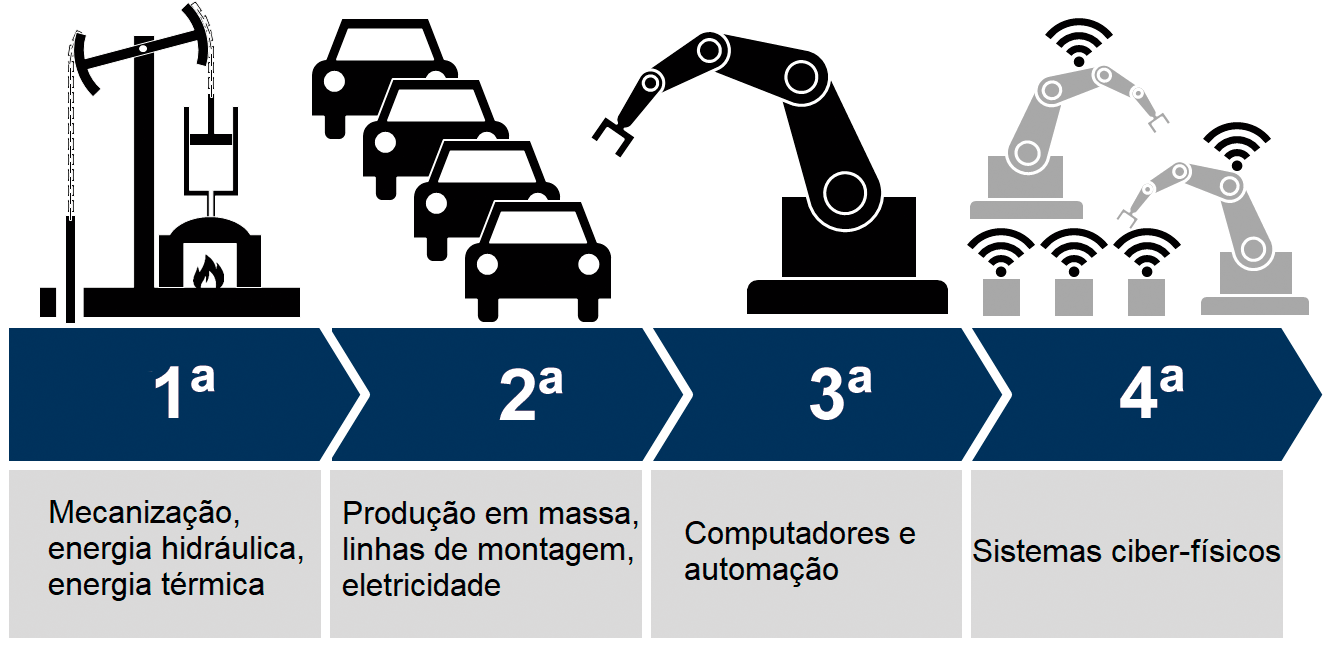
\includegraphics[width=0.7\textwidth]{i4.png}
	\end{figure}

	Princípios da I4.0:
	\begin{itemize}
		\item Interoperabilidade
		\item Transparência de informações
		\item Descentralização de decisões
		\item Assistência técnica
	\end{itemize}
	
\end{frame}
%---
\begin{frame}
	\frametitle{Memória digital do produto (MDP)}

	\begin{figure}[htb]
		\centering
		\caption{Coleta de dados do produto ao longo da cadeia de valores.}
		\label{fig:mdp}
		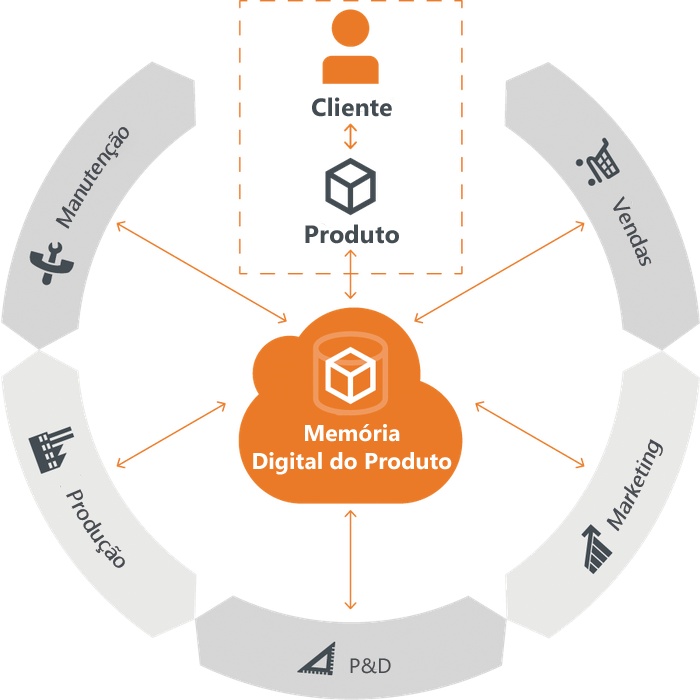
\includegraphics[width=0.6\textwidth]{mdp.png}
	\end{figure}
	 	
\end{frame}
%---
\begin{frame}
	\frametitle{Objetivos do trabalho}
	
	\begin{itemize}
		\item Elaboração de uma arquitetura orientada a serviços baseada no RAMI4.0
		\item Arquitetura para o compartilhamento da MDP ao longo da cadeia de suprimentos
		\item Integração do conceito de MDP ao RAMI4.0
		\item Mapeamento das operações de um Web Service ao RAMI4.0
		\item Proposta de estruturação dos dados da MDP
		\item Considerações do compartilhamento de informações do produto sobre o ciclo de vida do produto
	\end{itemize}

\end{frame}
%---
\begin{frame}
	\frametitle{Contribuição do trabalho}
	
	\begin{itemize}
		\item Refinamento do Modelo de Arquitetura de Referência para I4.0 (RAMI4.0)
		\item Padronização do formato de compartilhamento de informações dos ativos entre empresas
		\item Eficiência logística
	\end{itemize}
	
\end{frame}
%---
\begin{frame}
	\frametitle{Metodologia}
	
	\begin{figure}[htb]
		\centering
		\caption{Teorias, ferramentas e aplicações apontadas em diferentes fases do projeto de pesquisa.}
		\label{fig:metodologia-jensen-projeto}
		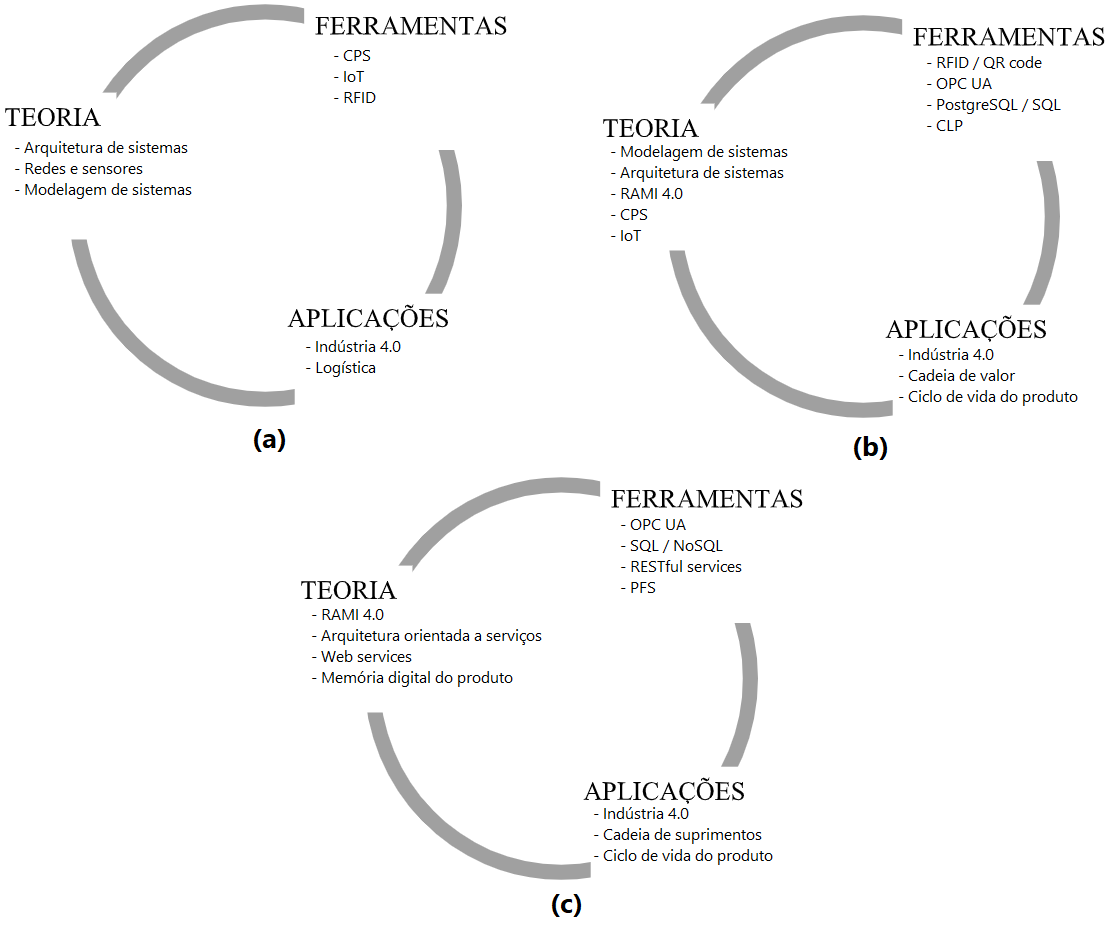
\includegraphics[width=0.7\textwidth]{metodologia-jensen-projeto.png}
	\end{figure}
	
\end{frame}

\iffalse
%------------------------------------------------
\section{Fundamentos}
%------------------------------------------------

\begin{frame}
	\frametitle{Fundamentação teórica}

	\begin{itemize}
		\item Indústria 4.0
		\item Logística \& Cadeia de Suprimentos
		\item Ciclo de vida do produto
		\item Memória digital do produto (MDP)
		\item Arquitetura orientada a serviços (SOA)
		\item Modelagem de sistemas
	\end{itemize}

\end{frame}
%---
\begin{frame}
	\frametitle{Indústria 4.0} - Conceitos
	
	\begin{block}{Conceito de I4.0 - Plattform Industrie 4.0 }
		Indústria 4.0 refere-se à rede inteligente de máquinas e processos para a indústria com a ajuda das Tecnologia da Informação e Comunicação (TIC).
	\end{block}

	Formas de se implementar redes empresariais inteligentes:
	
	\begin{itemize}
		\item Produção flexível
		\item Fábrica conversível
		\item Soluções orientadas ao consumidor
		\item Logística otimizada
		\item Uso de dados
		\item Economia circular com eficiência em recursos
	\end{itemize}
	
\end{frame}
%---
\begin{frame}
	\frametitle{Indústria 4.0 - RAMI4.0}
	
	\begin{figure}[htb]
		\centering
		\caption{Representação do RAMI4.0.}
		\label{fig:rami4}
		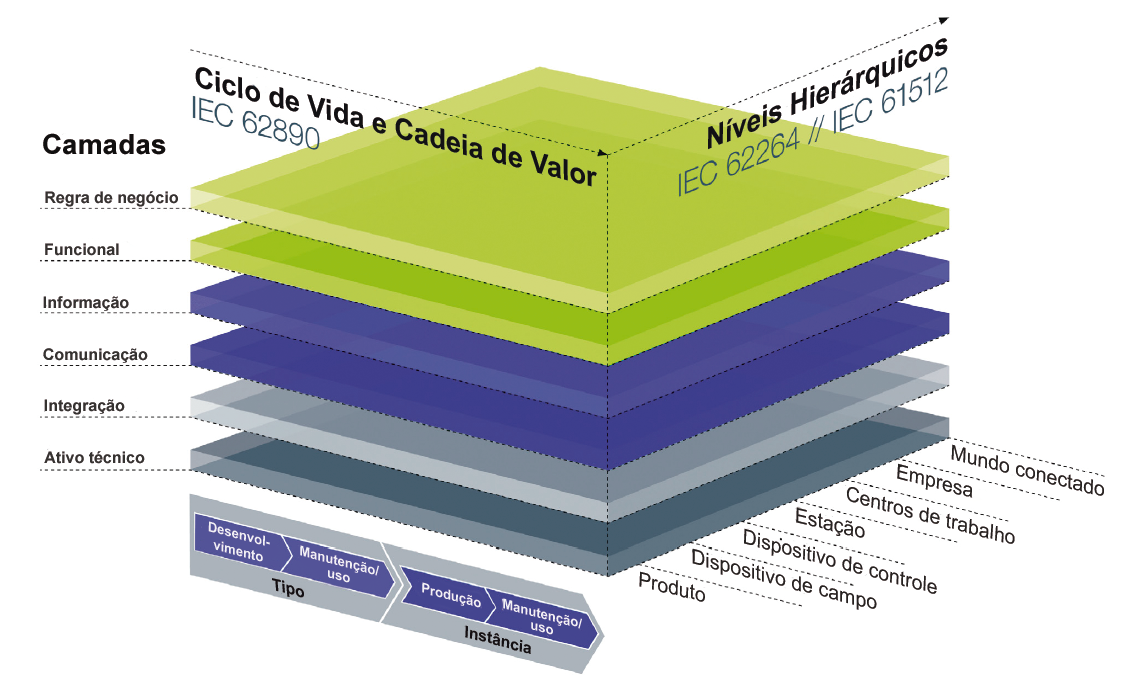
\includegraphics[width=1\textwidth]{rami4.png}
	\end{figure}
	
\end{frame}
%---
\begin{frame}
	\frametitle{Indústria 4.0 - AAS} 
	
	\begin{figure}[htb]
		\centering
		\caption{Representação do AAS como a parte virtual do Componente I4.0.}
		\label{fig:aas-rami}
		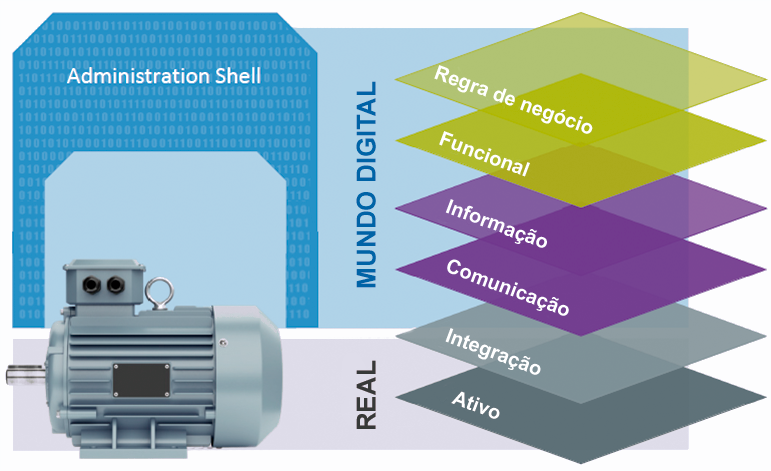
\includegraphics[width=0.8\textwidth]{aas-rami.png}
	\end{figure}
	
\end{frame}
%---
\begin{frame}
	\frametitle{Logística \& Cadeia de Suprimentos} 
	
	\begin{figure}[htb]
		\centering
		\caption{Exemplo de cadeia de suprimentos estendida.}
		\label{fig:cadeia-de-suprimentos}
		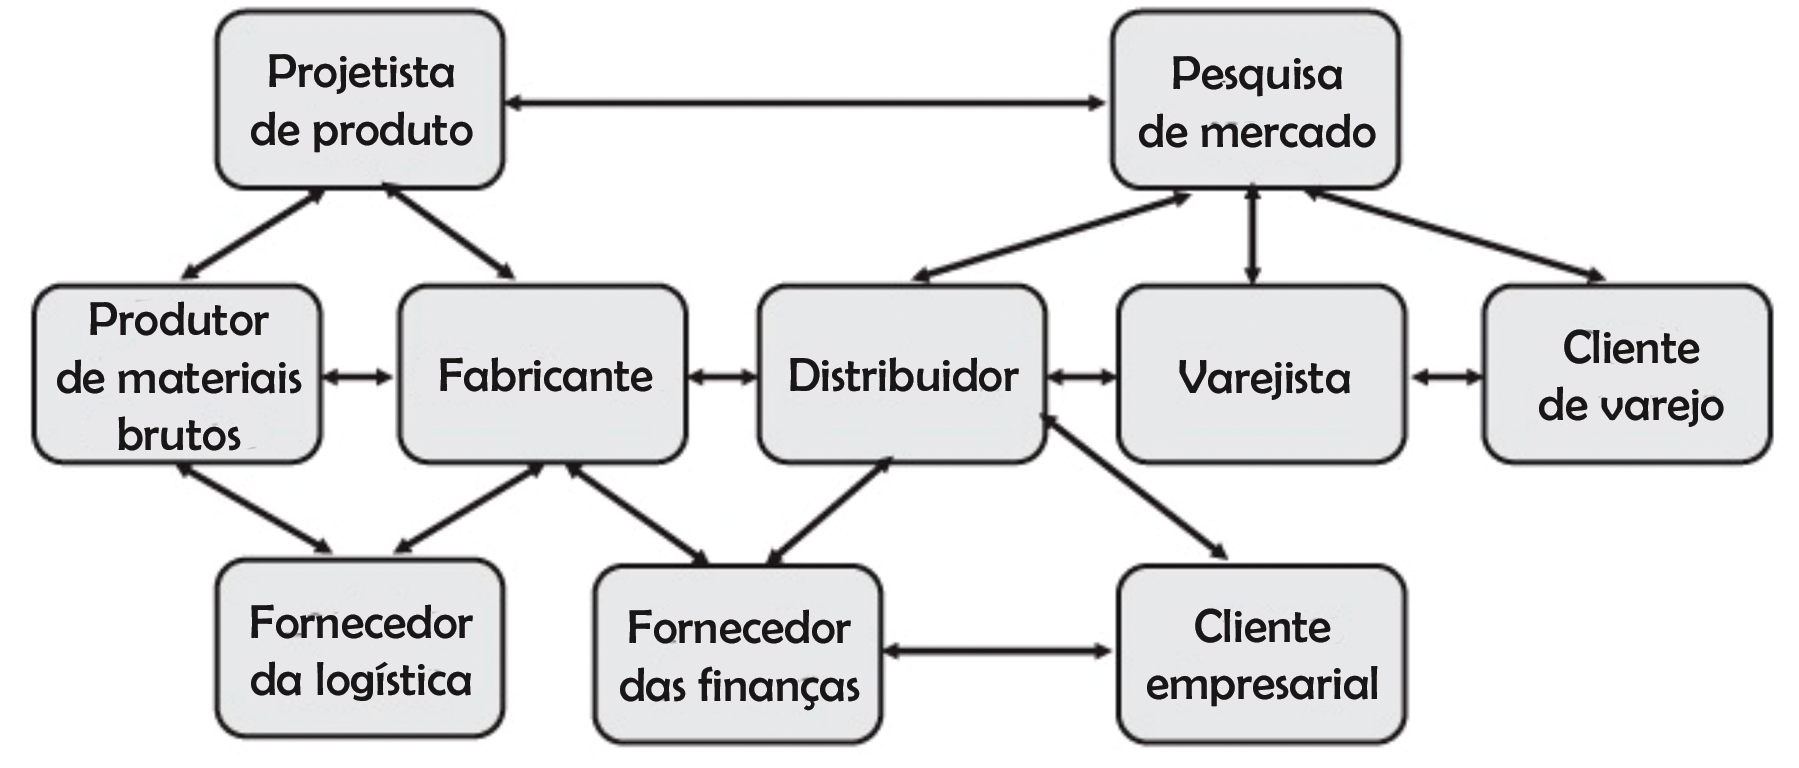
\includegraphics[width=1\textwidth]{cadeia-de-suprimentos.png}
	\end{figure}
	
\end{frame}
%---
\begin{frame}
	\frametitle{Logística \& Cadeia de Suprimentos - Logística 4.0}
	
	\begin{itemize}
		\item Maior integração entre os participantes da cadeia de suprimento
		\item Prazos de entrega menores
		\item Otimização de espaços e de custos de armazenagem
		\item Menor burocracia nos processos, elevando a produtividade e competitividade no mercado
		\item Geração de grande quantidade de dados como instrumentos de apoio nas tomadas de decisão
		\item Uso intensivo das Tecnologias de Informação e Comunicação (TIC)
	\end{itemize}
	
\end{frame}
%---
\begin{frame}
	\frametitle{Ciclo de vida do produto} 
	
	\begin{figure}[htb]
		\centering
		\caption{Modelo de ciclo de vida do produto com renovação do produto.}
		\label{fig:ciclo-de-vida-extensao}
		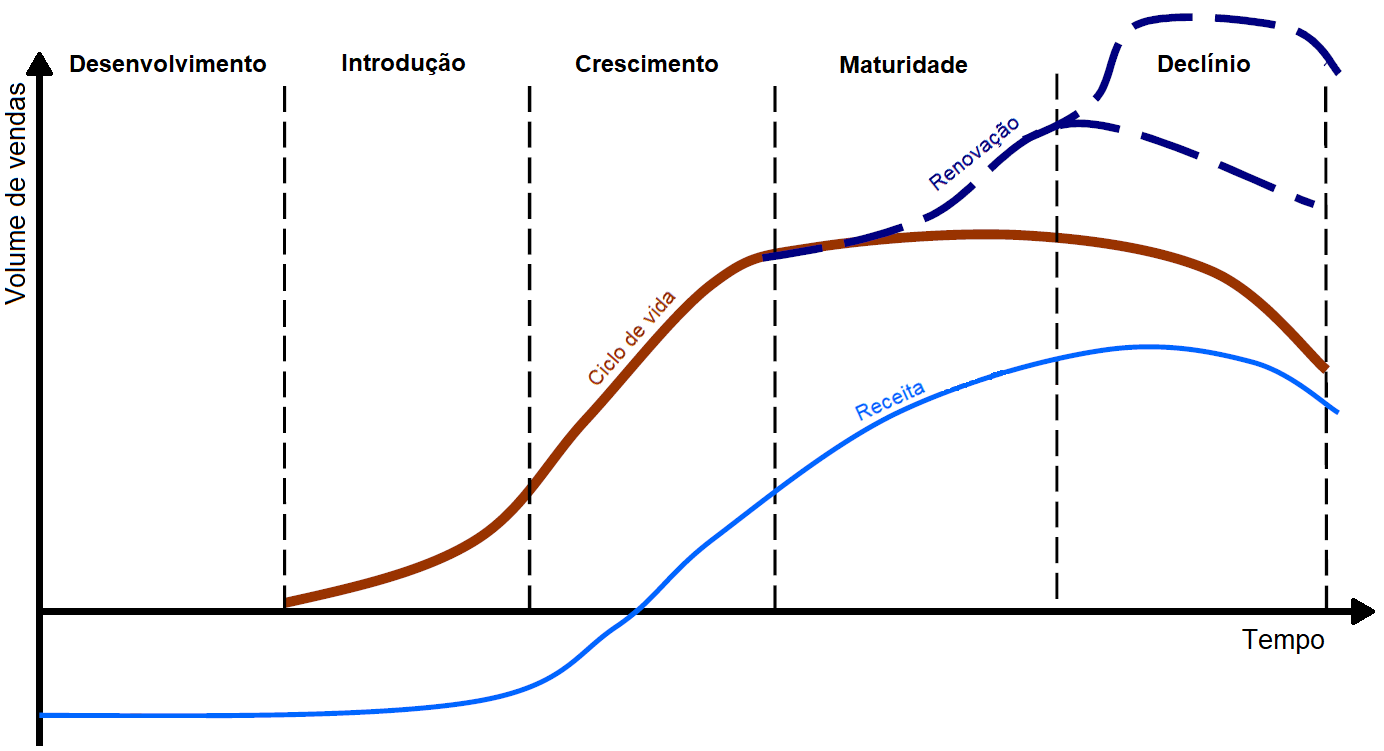
\includegraphics[width=1\textwidth]{ciclo-de-vida-extensao.png}
	\end{figure}
	
\end{frame}
%---
\begin{frame}
	\frametitle{Memória digital do produto} 
	
	\begin{itemize}
		\item Analogia a um ``diário'', contendo todas as informações do produto ao longo de seu ciclo de vida
		\item Sistemas que permitem a coleta de dados em todas as fases do ciclo de vida
		\item Compartilhamento de dados para as partes da cadeia de suprimentos
		\item Extração de valor a partir de dados (\textit{Big Data \& Data Analytics})
	\end{itemize}
	
\end{frame}
%---
\begin{frame}
	\frametitle{Arquitetura orientada a serviços} 
	
	\begin{figure}[htb]
		\centering
		\caption{Interconexão entre os elementos do sistema (a) com um \textit{middleware} e (b) sem um \textit{middleware}.}
		\label{fig:middleware}
		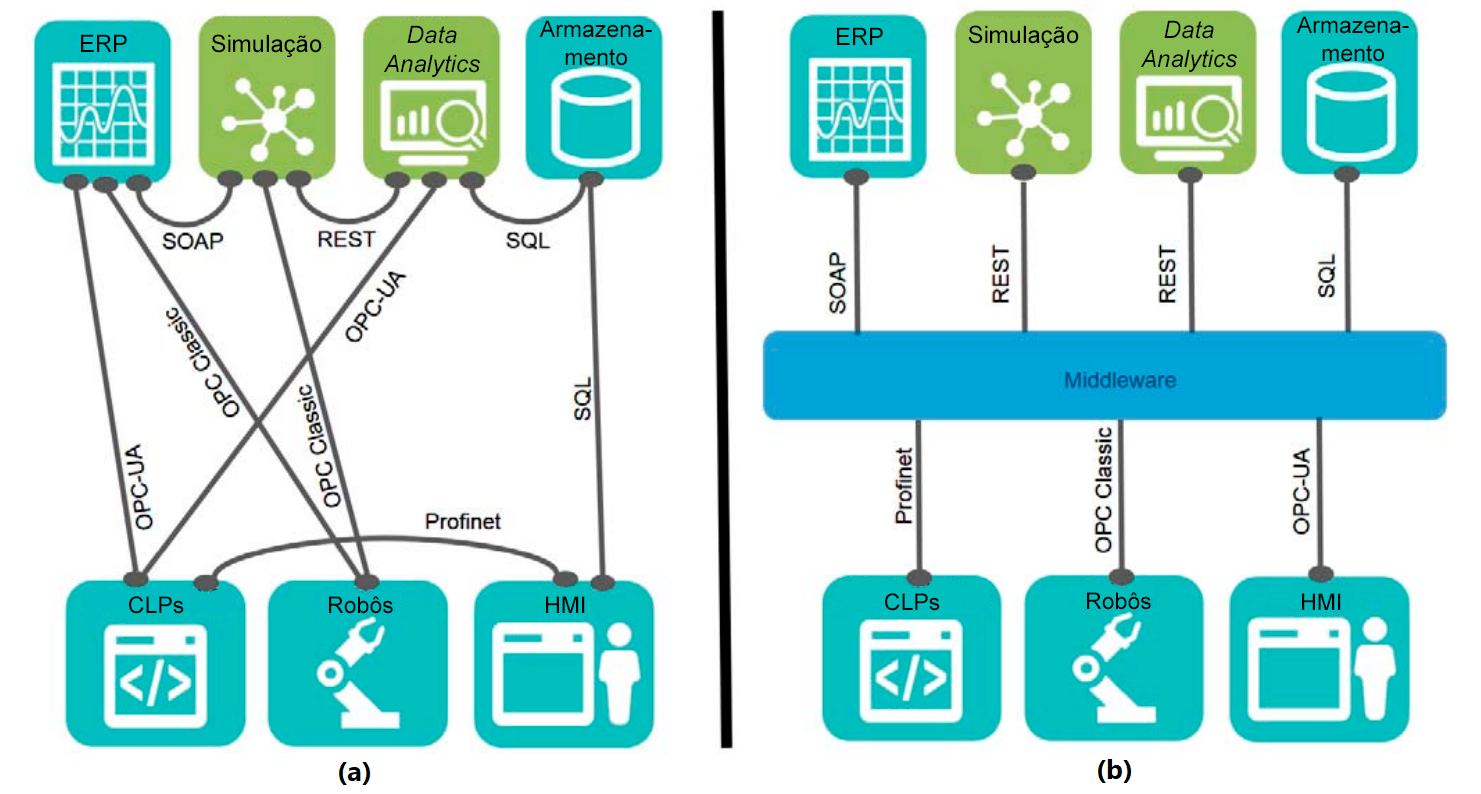
\includegraphics[width=0.9\textwidth]{middleware.png}
	\end{figure}
	
\end{frame}
%---
\begin{frame}
	\frametitle{Arquitetura orientada a serviços - Web Services} 
	
	\begin{figure}[htb]
		\centering
		\caption{Componentes de um WS e operações.}
		\label{fig:webservice-componentes}
		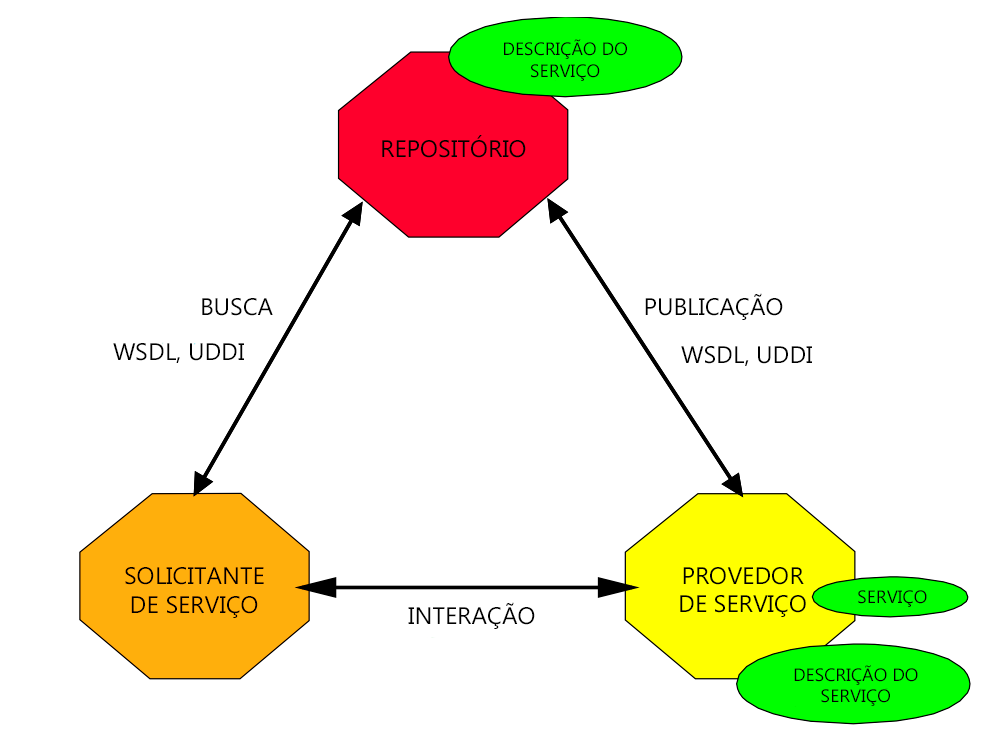
\includegraphics[width=0.8\textwidth]{webservice-componentes}
	\end{figure}
	
\end{frame}
%---
\begin{frame}
	\frametitle{Modelagem de sistemas} 
	
	\begin{block}{Conceito de sistema}
		Sistemas são um conjunto de elementos interdependentes de modo a formar um todo organizado. Também pode ser entendido como um conjunto de órgãos funcionais, componentes, entidades, partes ou elementos e as relações entre eles, com um objetivo geral a ser atingido.
	\end{block}

	\begin{block}{Sistemas logísticos}
		Um sistema pode ser definido como o conjunto de diferentes cadeias de suprimentos ligadas por meio de relacionamentos interorganizacionais, que fazem acontecer os fluxos envolvidos (de dinheiro, materiais, bens e informações).
		
	\end{block}
	
	Modelagem e análise dos sistemas
	
	\begin{itemize}
		\item Capturar e entender o funcionamento do sistema
		\item Entender as interações entre os atores do sistema
	\end{itemize}
	
\end{frame}
%---
\begin{frame}
	\frametitle{Modelagem de sistemas - PFS} 
	
	\begin{itemize}
		\item \textit{Production Flow Schema} (PFS)
		\item Modelagem, análise e controle de Sistema a Eventos Discretos (SED)
	\end{itemize}

	\begin{columns}[c] % The "c" option specifies centered vertical alignment while the "t" option is used for top vertical alignment
		\column{.5\textwidth} % Left column and width
		\begin{figure}[htb]
			\centering
			\caption{Elementos do PFS.}
			\label{fig:pfs-elementos}
			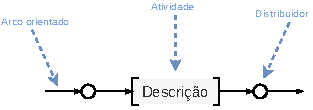
\includegraphics[width=1\textwidth]{pfs-elementos}
		\end{figure}
		
		\column{0.5\textwidth} % Right column and width]
		\begin{figure}[htb]
			\centering
			\caption{Tipos de fluxo no PFS.}
			\label{fig:pfs-fluxos}
			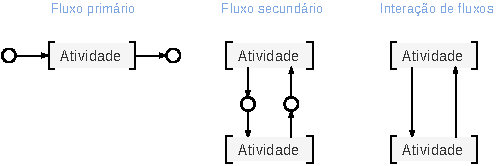
\includegraphics[width=1\textwidth]{pfs-fluxos}
		\end{figure}
		
	\end{columns}
	
\end{frame}
\fi

%------------------------------------------------
\section{Arquitetura}
%------------------------------------------------

\begin{frame}
	\frametitle{Componentes e Operações da Arquitetura}
	
	\begin{itemize}
		\item Arquitetura para o compartilhamento de informações do produto
		\item Garantir a interoperabilidade entre os membros da CS
		\item Compartilhamento de informações por meio de serviços (ou Web Services)
	\end{itemize}

	Componentes
	\begin{enumerate}
		\item AAS Servidor
		\item AAS Cliente
		\item AAS Repositório
	\end{enumerate}

	Operações
	\begin{enumerate}
		\item AAS Publicação
		\item AAS Busca
		\item AAS Interação
	\end{enumerate}
	
\end{frame}
%---
\begin{frame}
	\frametitle{Dinâmica dos componentes e operações da arquitetura}
	
	\begin{figure}[htb]
		\centering
		\caption{Componentes e operações do WS.}
		\label{fig:aas-ws}
		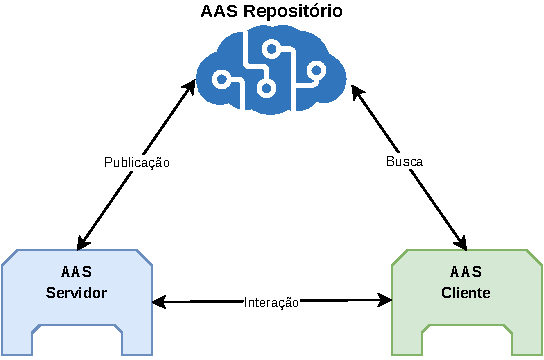
\includegraphics[width=0.8\textwidth]{aas-ws}
	\end{figure}
	
\end{frame}
%---
\begin{frame}
	\frametitle{Componentes}

	\begin{table}[htb]
		\centering
		\caption{Componentes da arquitetura para a I4.0.}
		\label{tab:componentes-ws}
		\resizebox{\textwidth}{!}{	
		\begin{tabular}{p{3cm}p{12cm}}
			\hline
			\textbf{Componente}
			& \textbf{Descrição} \\ 
			
			\hline
			AAS Servidor
			& O AAS Servidor é a conexão direta com o ativo. Este AAS extrai as informações sobre seu ativo para sua própria MDP para que assim possam ser disponibilizadas na rede. Cada submodelo do AAS representa um conjunto de informações e serviços semelhantes agrupados. \\
			
			\hline
			AAS Cliente
			& O AAS Cliente é a parte que irá consumir as informações disponibilizadas pelo AAS Servidor. O cliente representa cada uma das partes envolvidas na cadeia de suprimentos. Pode representar uma instituição, uma pessoa física ou até mesmo uma outra máquina/produto. \\
			
			\hline
			AAS Repositório
			& O repositório é o componente que recebe, armazena e disponibiliza informações de descrição sobre todos os serviços disponíveis no mundo conectado. O AAS recebe operações de ``publicação'' por parte do AAS Servidor e operações de ``busca'' por parte do AAS Cliente. O Repositório não atua como canal de comunicação entre AAS Cliente e Servidor, mas apenas fornece informações necessárias para que ambos os AAS possam se comunicar diretamente por meio da operação de ``interação''. \\
			
			\hline
		\end{tabular}
		}
	\end{table}
	
\end{frame}
%---
\begin{frame}
	\frametitle{Operações}
	
	\begin{table}[htb]
		\centering
		\caption{Operações do WS para a I4.0.}
		\label{tab:operacoes-ws}
		\resizebox{\textwidth}{!}{
		\begin{tabular}{p{3cm}p{12cm}}
			\hline
			\textbf{Operação}
			& \textbf{Descrição} \\ 
			
			\hline
			Publicação
			& Ação tomada pelo AAS Servidor sempre que este componente queira anunciar um serviço para que possa ser descoberto. Nesta operação, o AAS Servidor envia uma lista de seus serviços ofertados e a descrição de cada um desses serviços. Esta lista é recebida e armazenada pelo AAS Repositório, que a disponibiliza para acesso público. \\
			
			\hline
			Busca
			& Ação tomada pelo AAS Cliente sempre que este precisa consultar serviços de seu interesse. Nesta operação o AAS Cliente faz uma solicitação ao AAS Repositório com os parâmetros que definem o tipo e as restrições do serviço desejado. A operação de busca engloba também o fluxo contrário de informações, que é o envio da resposta da solicitação do AAS Repositório para o AAS Cliente. \\
			
			\hline
			Interação
			& Ação tomada pelo AAS Cliente sempre que este deseja invocar um serviço. O AAS Cliente estabelece uma conexão direta com o AAS Servidor e consome o determinado serviço solicitado. A operação de interação normalmente é feita após o recebimento da lista de descrição de serviços por parte do AAS Repositório, porém a interação pode ser feita diretamente caso o AAS Cliente já possua informações necessárias para o estabelecimento da conexão.  \\
			
			\hline
		\end{tabular}
		}
	\end{table}
	
	
\end{frame}
%---
\begin{frame}
	\frametitle{Componentes e Operações}
	
	\begin{figure}[htb]
		\centering
		\caption{Diagrama PFS das operações do WS.}
		\label{fig:pfs-ws}
		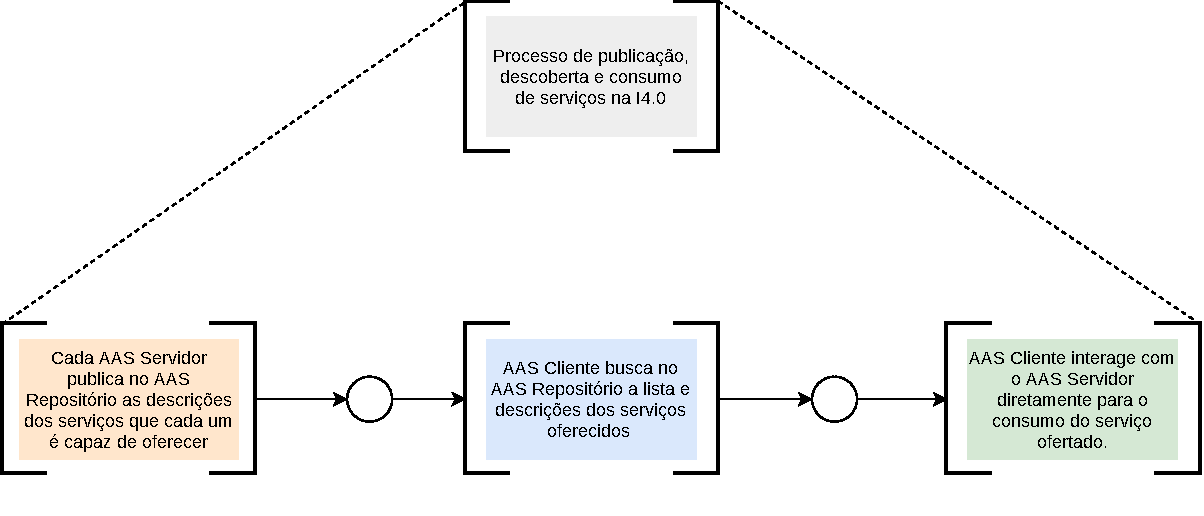
\includegraphics[width=1\textwidth]{pfs-ws}
	\end{figure}
	
\end{frame}
%---
\begin{frame}
	\frametitle{Conteúdo da MDP - AAS Repositório}
	
	\begin{table}[htb]
		\centering
		\caption{Proposta de metamodelo para a MDP do repositório.}
		\label{tab:mdp-repositorio}
		\resizebox{0.75\textwidth}{!}{
		\begin{tabular}{p{3cm}p{12cm}}
			\hline
			\textbf{Propriedade}
			& \textbf{Descrição} \\ 
			
			\hline
			ID do AAS servidor
			& Tem a função de distinguir exclusivamente os AASs provedores de serviços e todos seus elementos no mundo conectado da I4.0. Alguns tipos possíveis de identificadores são: IRDI, IRI e UUID. O ID do AAS servidor é uma referência ao AAS Repositório e a todos os demais AASs que solicitarem a descrição dos serviços. \\
			
			\hline
			ID do serviço
			& Identificação exclusiva do serviço para a sua identificação única entre todos os repositórios. O ID do serviço pode ser derivado do próprio ID do AAS servidor com identificações extra do ID dentro do AAS (E.g., ID\_MODELO.SERVIÇO\_001). \\
			
			\hline
			Descrição do AAS provedor
			& Breve descrição sobre o AAS servidor e suas funções. \\
			
			\hline
			Protocolos de comunicação e padrões de API
			& Definição dos protocolos de comunicação suportados pelo fornecedor daquele serviço, como, por exemplo, HTTP, MQTT, etc; assim como as especificações do padrão para a comunicação via API como, por exemplo, REST, SOAP, GraphQL, etc.   \\
			
			\hline
			Formato de intercâmbio
			& Formato de arquivo de intercâmbio de informações. Ex.: json, xml, yaml, aasx, etc.  \\
			
			\hline
			\textit{Timestamp} da inserção do serviço no repositório
			& Data e hora de inserção do serviço ao repositório. \\
			
			\hline
			Indicação de disponibilidade
			& Chave booleana indicando se o AAS servidor atualmente suporta requisições. Esta propriedade pode estar desatualizada caso o AAS Servidor sofra uma falha de comunicação. Em outros casos, o AAS Servidor pode voluntariamente indicar ao repositório que temporariamente não processará solicitações de serviços. \\
			
			\hline
			Quality of Service (QoS)
			
			& A métrica de qualidade de serviço (QoT) fornece indicadores sobre a qualidade do serviço prestado por um determinado AAS. O tempo médio de resposta do serviço baseado no tempo de resposta observado por diversas requisições executadas e a disponibilidade do AAS quando solicitado são índices que contribuição do QoS. Um índice para serviços de qualidade mais subjetiva pode ser criado baseado em avaliações de AAS Clientes que já consumiram o serviço.\\
			
			\hline
			Descrição do serviço
			& Descrição sobre o funcionamento do serviço juntamente com o tipo de resposta esperado.  \\			
			\hline
		\end{tabular}
		}

	\end{table}
	
\end{frame}
%---
\begin{frame}
	\frametitle{Conteúdo da MDP - AAS Servidor}
	
	\begin{table}[htb]
		\centering
		\caption{Proposta de metamodelo para a MDP do servidor.}
		\label{tab:mdp-servidor}
		\resizebox{1\textwidth}{!}{
		\begin{tabular}{p{4cm}p{11cm}}
			\hline
			\textbf{Propriedade/Função}
			& \textbf{Descrição} \\ 
			
			\hline
			ID do serviço
			& Identificação exclusiva do serviço para a sua identificação única entre todos os repositórios. \\
			
			\hline
			Extração de dados dos submodelos
			& Função que retorna os dados solicitados pelo serviço. \\
			
			\hline
			Organização dos dados
			& Funções de estruturação dos dados ao formato solicitado pelo serviço, nesta fase pode haver também funções de limpeza dos dados brutos extraídos dos submodelos. \\
			
			\hline
			\textit{Quality of Service} (QoS)
			& Função para cálculo e armazenamento do índice de qualidade de serviço (QoS) com base em métricas sobre serviços já prestados e avaliações de AAS clientes que já consumiram o serviço. \\
			
			\hline
			Atualização da descrição do serviço no repositório
			& Função que envia ao repositório da empresa a descrição atualizada dos serviços. \\
			
			\hline
			Repositório
			& Referência ao repositório da empresa onde o ativo se encontra. \\			
			\hline
		\end{tabular}
		}
	\end{table}
	
\end{frame}
%---
\begin{frame}
	\frametitle{Detalhamento das partes do AAS}
	
	\begin{figure}[htb]
		\centering
		\caption{Estrutura do AAS com seus submodelos e a MDP.}
		\label{fig:estrutura-aas}
		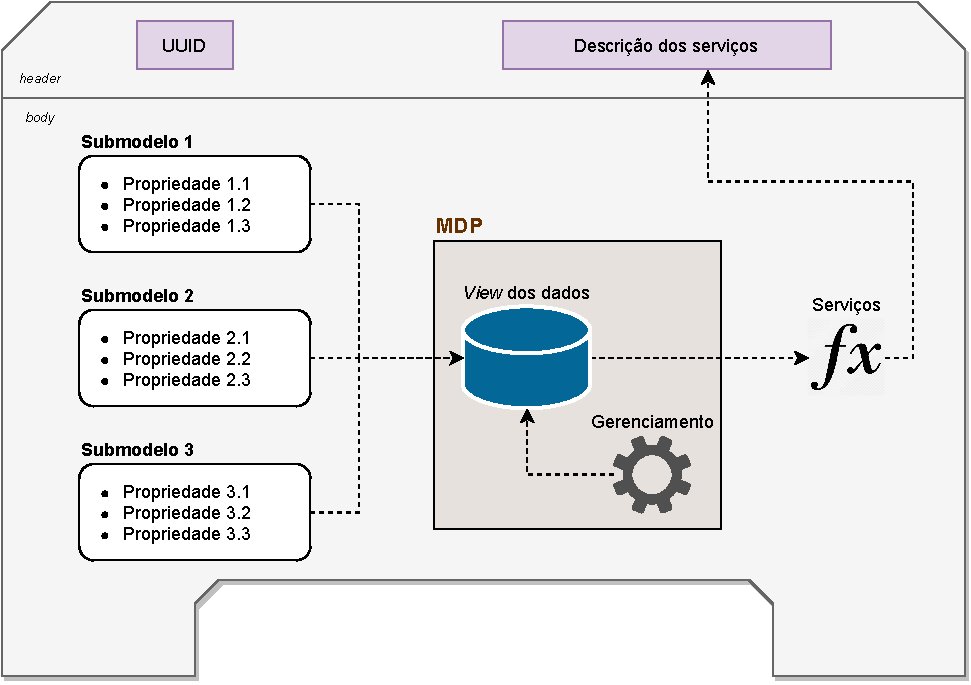
\includegraphics[width=0.8\textwidth]{estrutura-aas}
	\end{figure}
	
\end{frame}
%---
\begin{frame}
	\frametitle{Dinâmica dos serviços - Múltiplos elos}
	
	\begin{figure}[htb]
		\centering
		\caption{Exemplificação das operações de publicação e busca com múltiplos clientes.}
		\label{fig:webservice-multielo}
		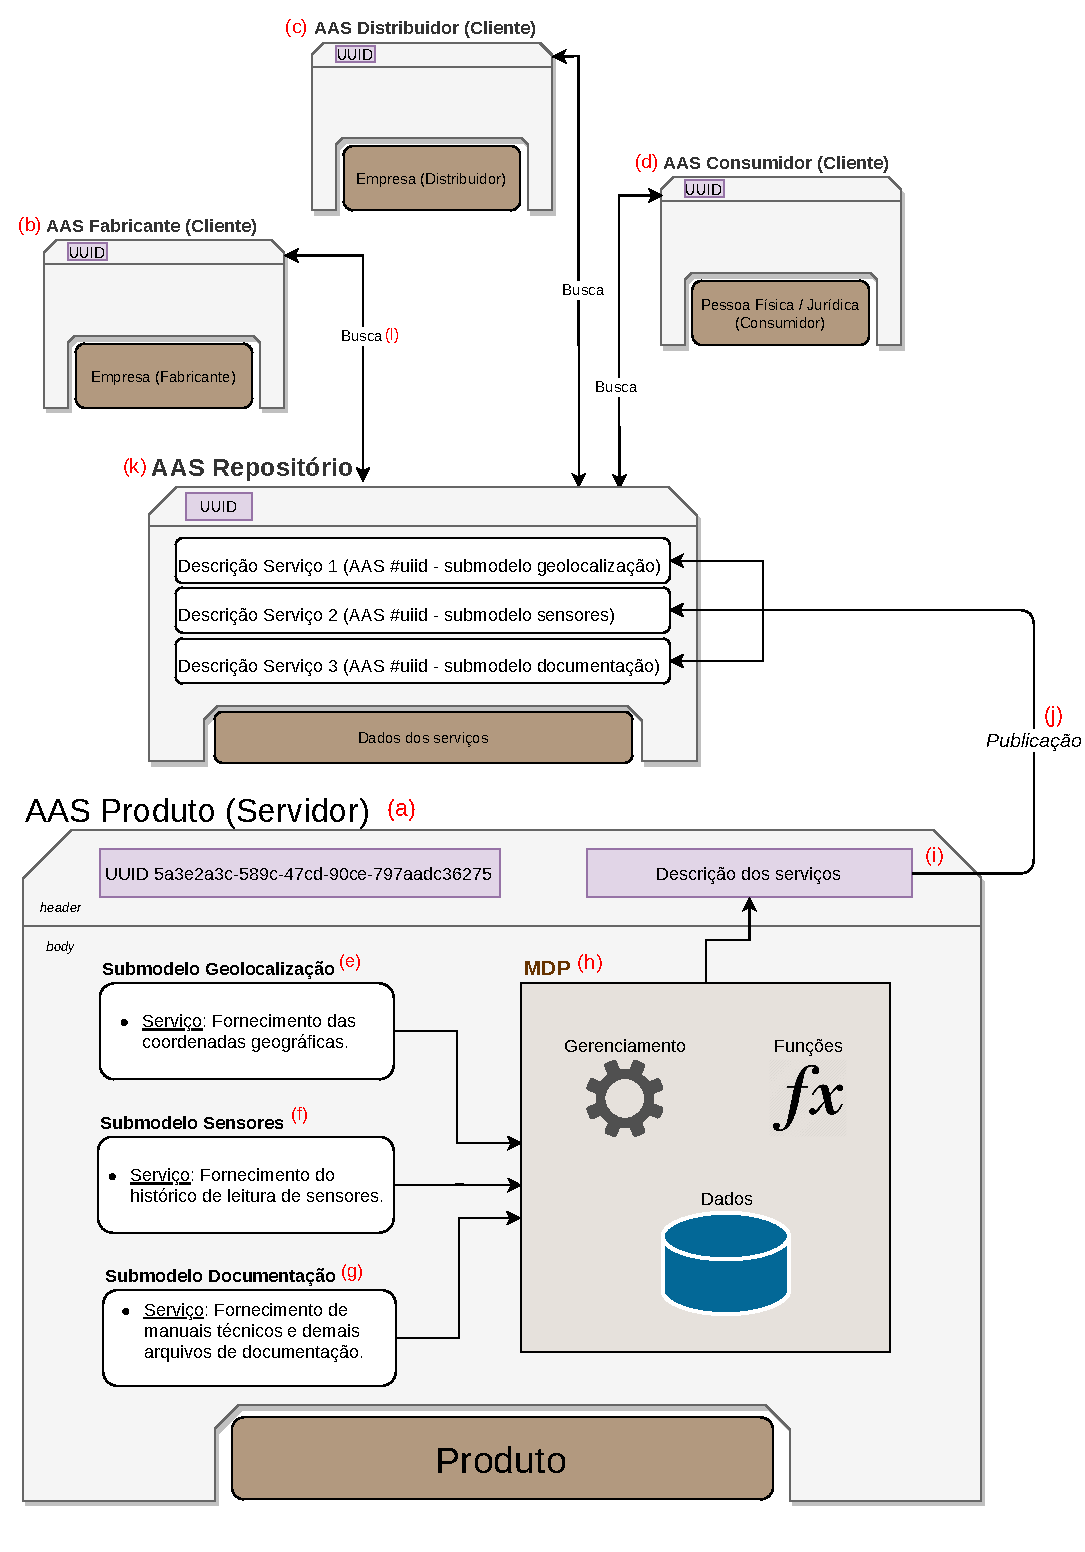
\includegraphics[width=1\textwidth]{webservice-multielo}
	\end{figure}
	
\end{frame}
%---
\begin{frame}
	\frametitle{Dinâmica dos serviços - Múltiplos produtos}
	
	\begin{figure}[htb]
		\centering
		\caption{Exemplificação das operações de publicação e busca com múltiplos produtos.}
		\label{fig:webservice-multiproduto}
		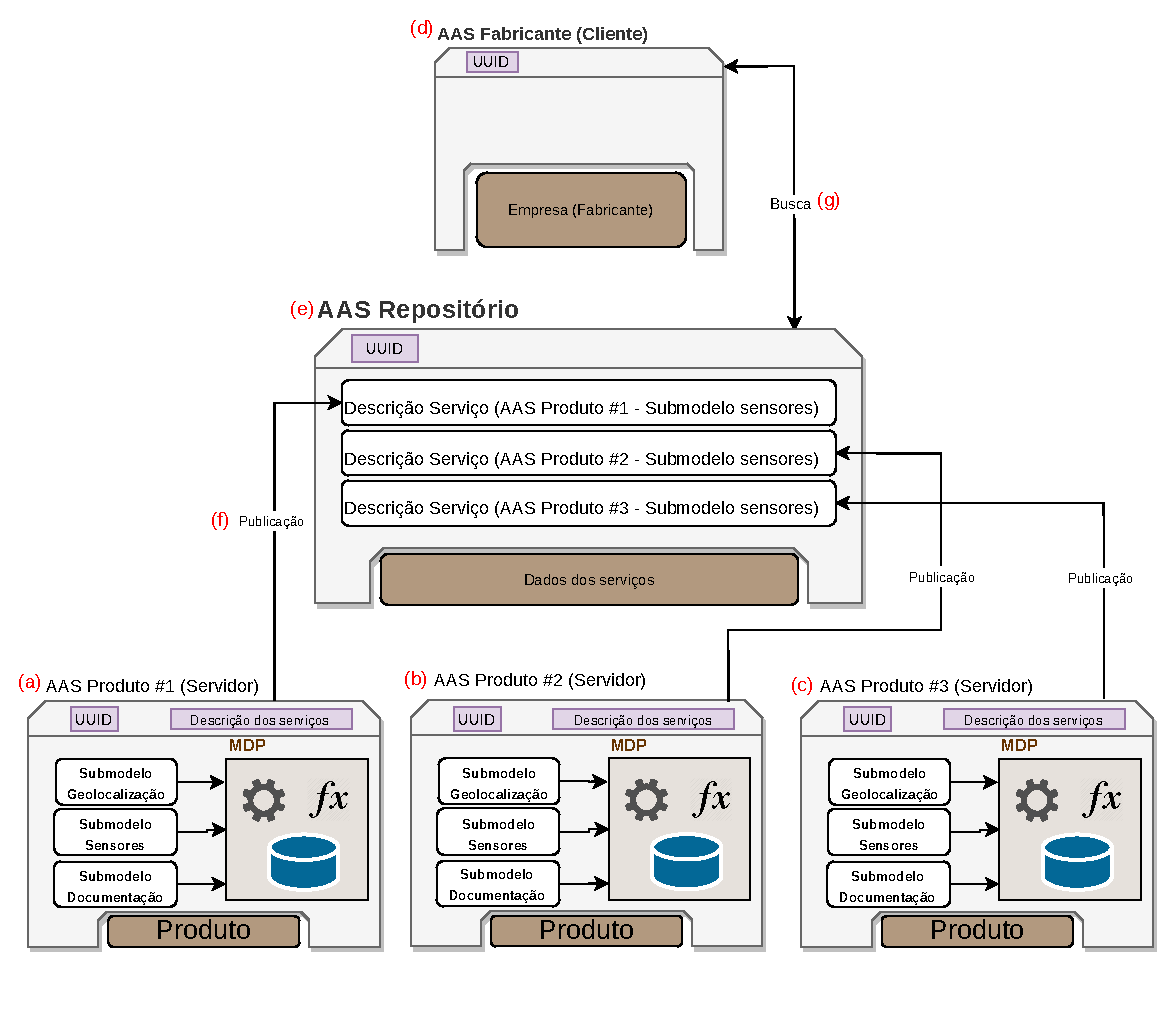
\includegraphics[width=0.7\textwidth]{webservice-multiproduto}
	\end{figure}
	
\end{frame}
%---
\begin{frame}
	\frametitle{Descrição das camadas do RAMI4.0}
	
	\begin{itemize}
		\item \textbf{Ativo}: Pessoas e empresas (cliente), produtos (servidor) e WSDs (repositório); 
		\item \textbf{Integração}: Virtualização das informações, protocolos de transferência de dados (Ethernet, 5G, Wi-Fi, etc); 
		\item \textbf{Comunicação}: Protocolos de comunicação vertical (OPC UA); 
		\item \textbf{Informação}: Controle de acesso / autenticação, análise de dados, armazenamento, descrição dos serviços (virtual);
		\item \textbf{Funcional}: Serviços de compartilhamento de informações, protocolos de comunicação horizontal (HTTPS, MQTT, etc), interface horizontal entre AASs; 
		\item \textbf{Regra de negócio}: Restrições legais, políticas de privacidade.
	\end{itemize}
	
\end{frame}
%---
\begin{frame}
	\frametitle{Descrição das camadas do RAMI4.0}
	
	\begin{figure}[H]
		\centering
		\caption{Camadas do RAMI4.0 com os elementos da arquitetura.}
		\label{fig:webservice-rami}
		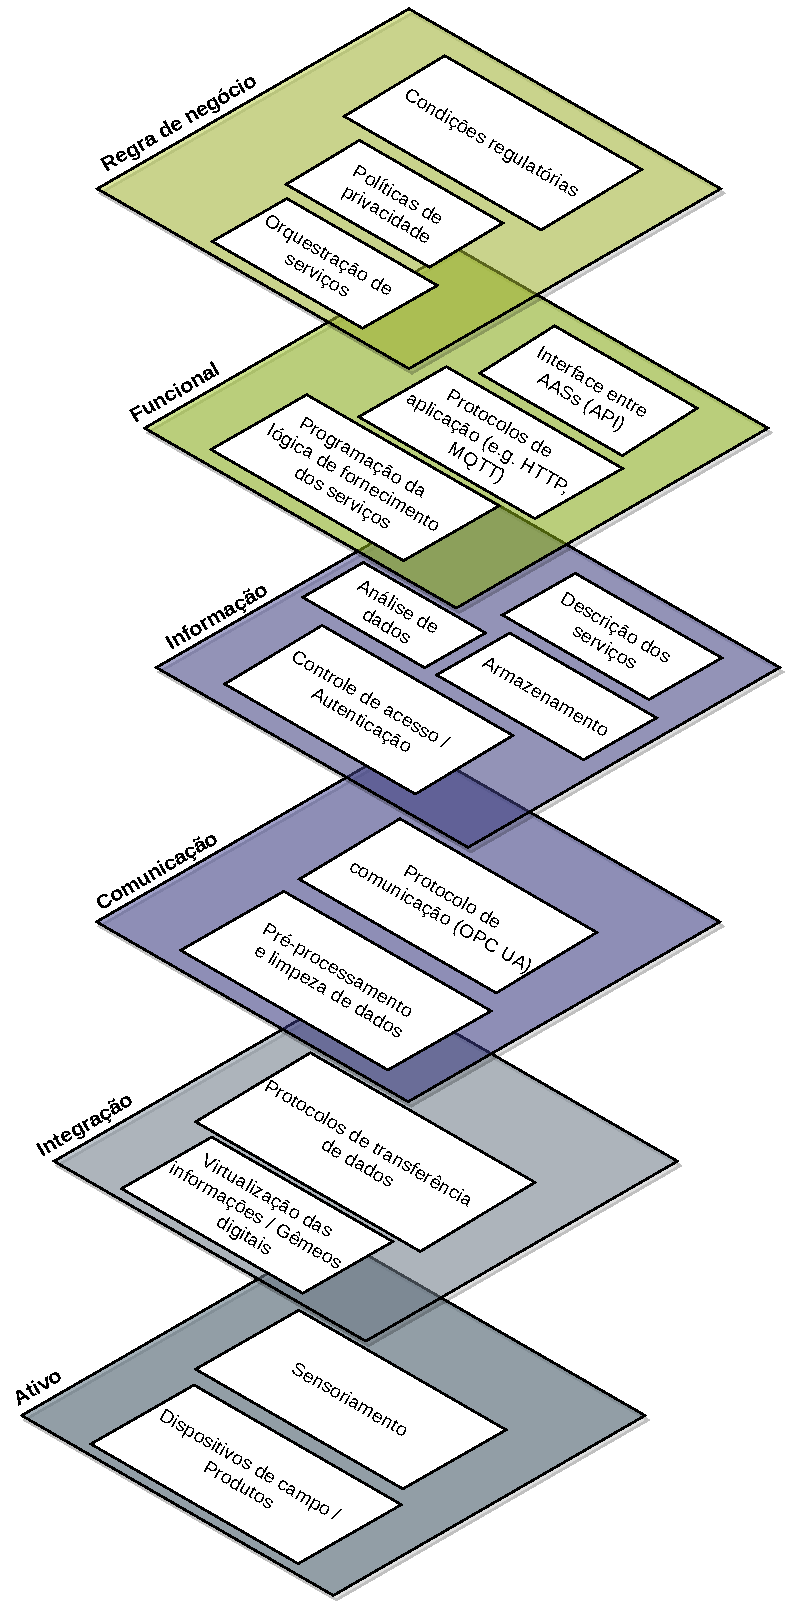
\includegraphics[width=0.8\textwidth]{webservice-rami}
	\end{figure}
	
\end{frame}
%---
\begin{frame}
	\frametitle{Mapeamento no RAMI4.0 - Publicação}
	
	\begin{figure}[htb]
		\centering
		\caption{Diagrama PFS da operação de publicação.}
		\label{fig:rami-publicacao}
		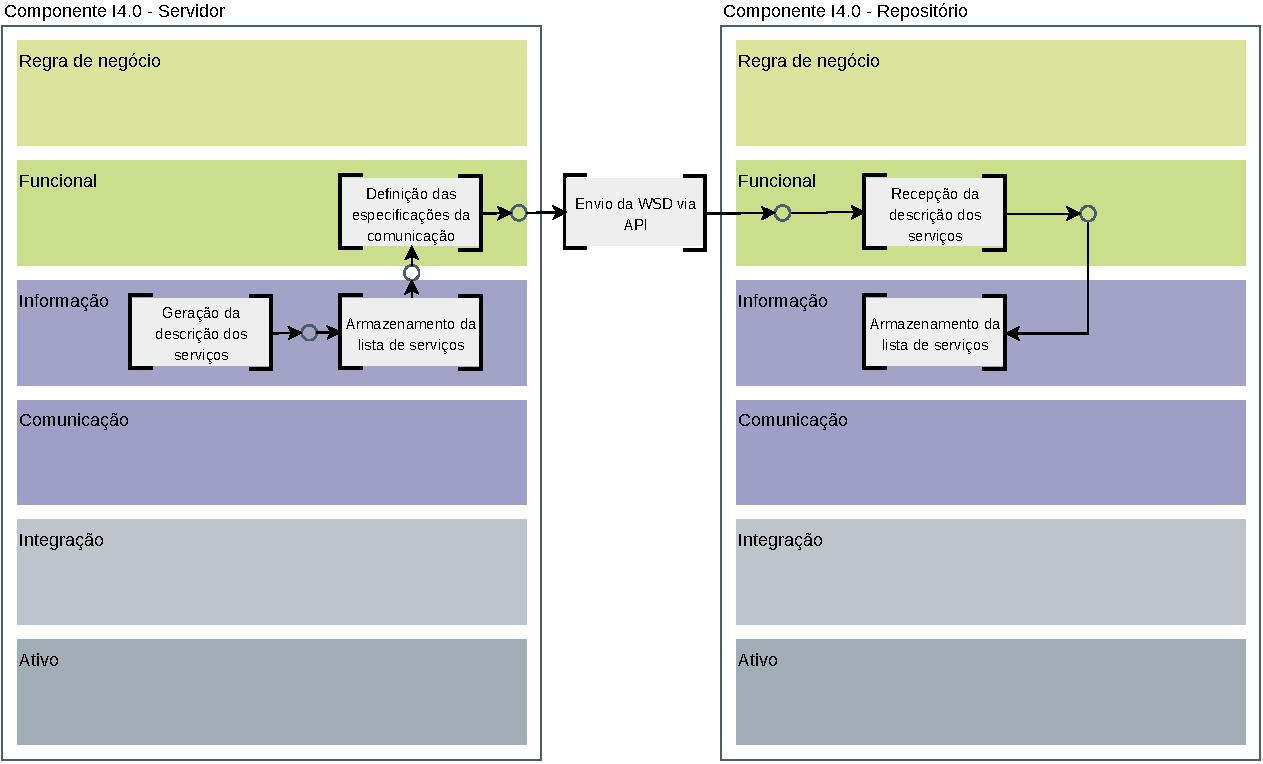
\includegraphics[width=1\textwidth]{rami-publicacao}
	\end{figure}
	
\end{frame}
%---
\begin{frame}
	\frametitle{Mapeamento no RAMI4.0 - Busca (Requisição)}
	
	\begin{figure}[htb]
		\centering
		\caption{Diagrama PFS da requisição em uma operação de busca.}
		\label{fig:rami-busca-requisicao}
		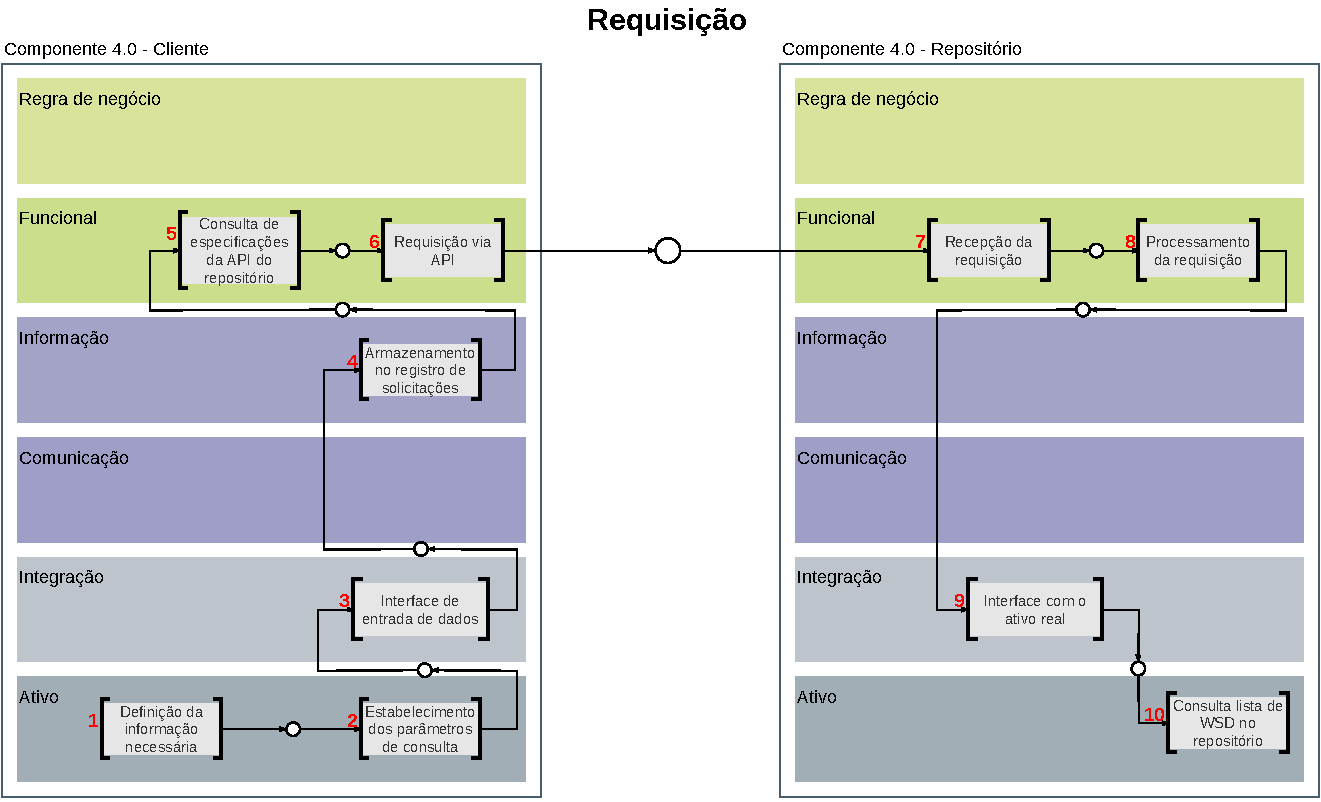
\includegraphics[width=0.9\textwidth]{rami-busca-requisicao}

	\end{figure}
	
\end{frame}
%---
\begin{frame}
	\frametitle{Mapeamento no RAMI4.0 - Busca (Resposta)}
	
	\begin{figure}[htb]
		\centering
		\caption{Diagrama PFS da resposta em uma operação de busca.}
		\label{fig:rami-busca-resposta}
		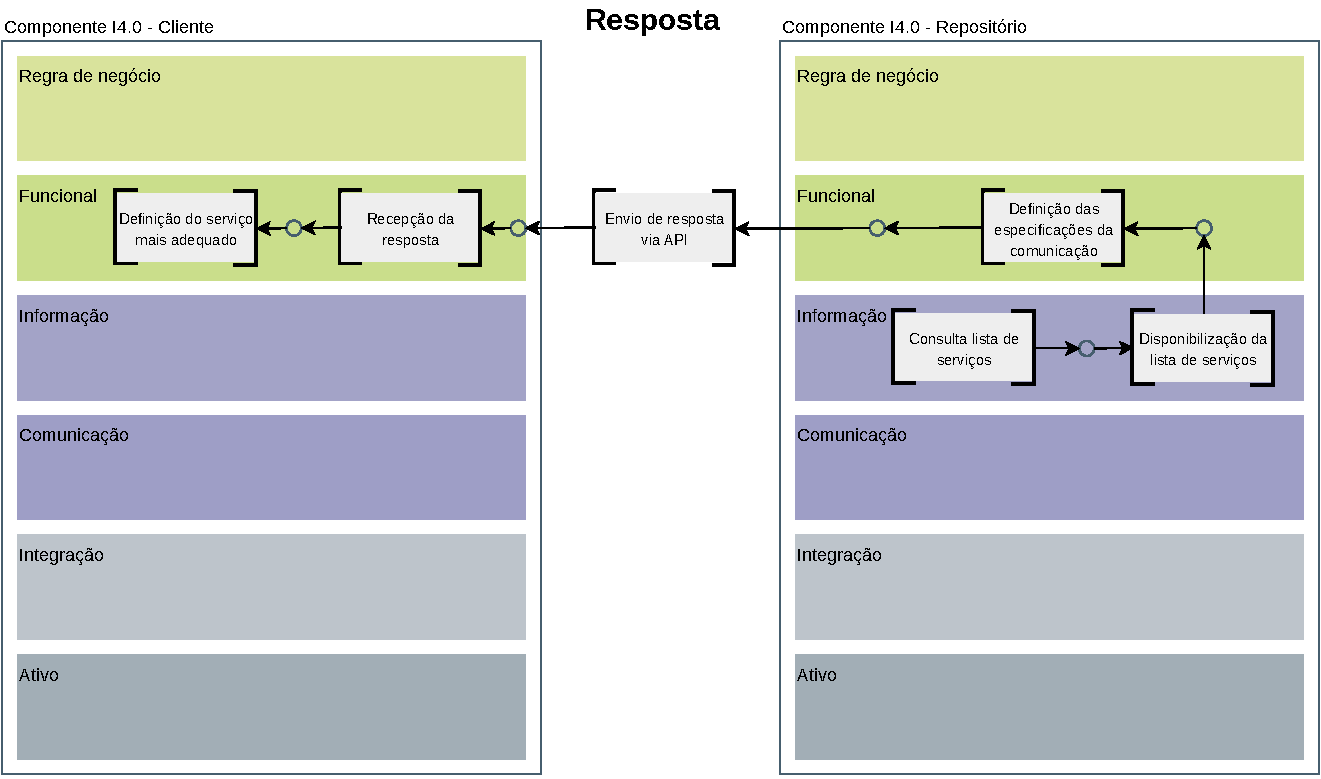
\includegraphics[width=0.9\textwidth]{rami-busca-resposta}

	\end{figure}

\end{frame}
%---
\begin{frame}
	\frametitle{Mapeamento no RAMI4.0 - Interação (Requisição)}
	
	\begin{figure}[htb]
		\centering
		\caption{Diagrama PFS da requisição de um serviço em uma operação de interação.}
		\label{fig:rami-interacao-requisicao}
		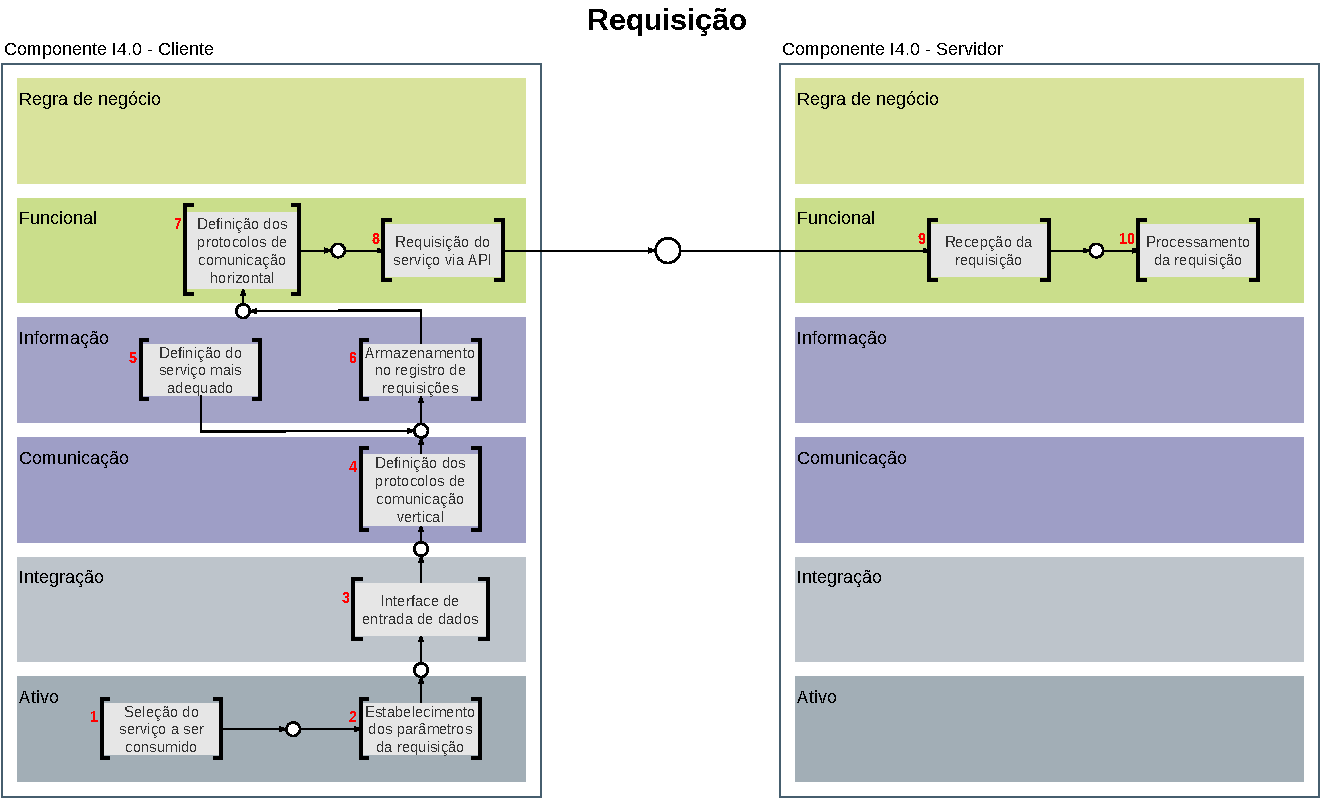
\includegraphics[width=0.9\textwidth]{rami-interacao-requisicao}
	
	\end{figure}
	
\end{frame}
%---
\begin{frame}
	\frametitle{Mapeamento no RAMI4.0 - Interação (Resposta)}
	
	\begin{figure}[htb]
		\centering
		\caption{Diagrama PFS da resposta de um serviço em uma operação de interação.}
		\label{fig:rami-interacao-resposta}
		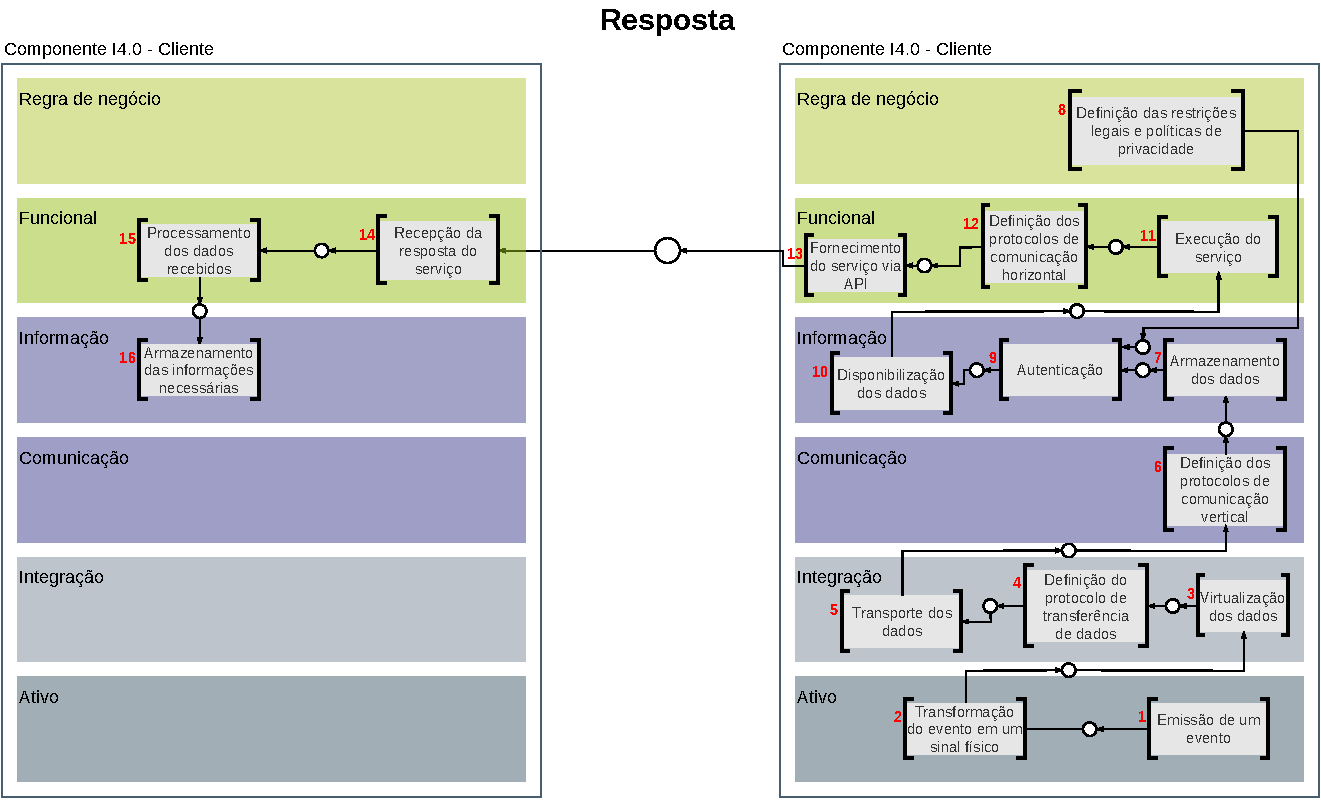
\includegraphics[width=0.9\textwidth]{rami-interacao-resposta}

	\end{figure}
	
\end{frame}

%------------------------------------------------
\section{Ciclo de vida}
%------------------------------------------------

\begin{frame}
	\frametitle{Ciclo de vida do produto}
	
	\begin{itemize}
		\item Impacto do amplo compartilhamento da MDP ao longo da CS
		\item Surgimento de novos modelos de negócio baseados em dados (\textit{data-driven})
		\item Atribuições de cada AAS em sua fase ``tipo'' e sua fase ``instância''
	\end{itemize}
	
\end{frame}
%---
\begin{frame}
	\frametitle{Extensão do ciclo de vida do produto segundo a I4.0}
	
	\begin{figure}[htb!]
		\centering
		\caption{Ciclo de vida do produto.}
		\label{fig:aas-lifecycle}
		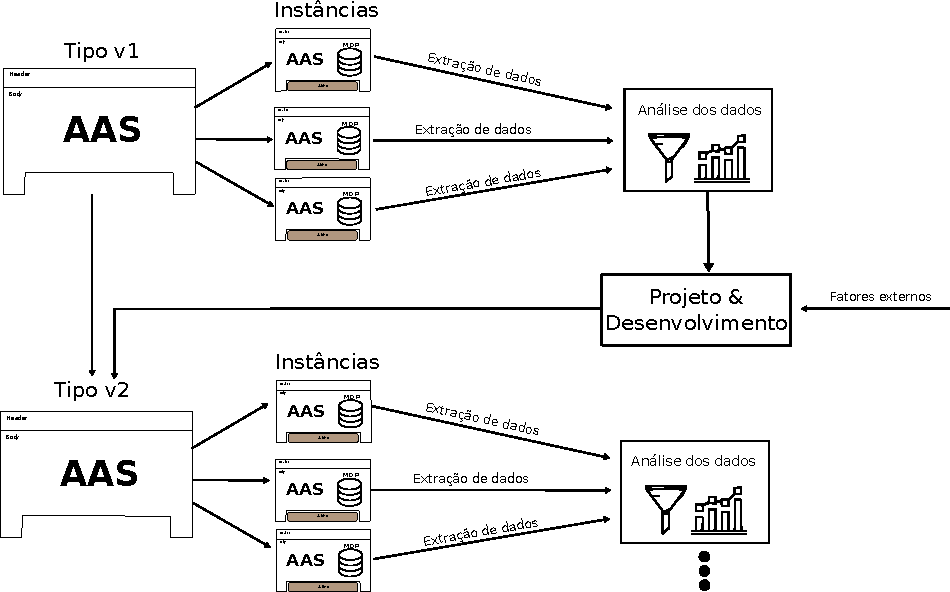
\includegraphics[width=0.9\textwidth]{aas-lifecycle}
	\end{figure}
	
\end{frame}
%---
\begin{frame}
	\frametitle{A MDP na fase ``tipo''}
	
	A análise de dados da MDP possibilita o aprimoramento do ``tipo'' do produto das seguintes maneiras:
	
	\begin{itemize}
		\item Identificação e reparo de falhas de projeto;
		\item Adição de novas funcionalidades ao produto;
		\item Melhoria da experiência do cliente/operador com o produto;
		\item Geração de indicadores de sustentabilidade.
	\end{itemize}
	
\end{frame}
%---
\begin{frame}
	\frametitle{Extração de informações pela MDP na fase ``tipo''}
	
		\begin{table}[htb]
		\centering
		\caption{Possíveis informações e respectivos submodelos para o aprimoramento do projeto do produto.}
		\label{tab:produto-tipo}
		\resizebox{1\textwidth}{!}{
		\begin{tabular}{p{4cm}p{3cm}p{3cm}p{4cm}}
			
			\hline
			\textbf{Informação}
			& \textbf{Submodelo}
			& \textbf{Cliente}
			& \textbf{Leitura}	
			\\ 
			
			\hline
			Histórico de leitura de sensores dos componentes
			& Leitura de sensores
			& Fabricante / Técnico de manutenção
			& Automática (E.g, a cada 6 horas)
			\\
			
			\hline
			Índice de disponibilidade, eficiência e qualidade do produto
			& Eficiência Global do Equipamento (OEE)
			& Fabricante / Gestor
			& Automática, sob solicitação
			\\
			
			\hline
			Volume de emissão de gases do efeito estufa
			& Pegada ambiental
			& Fabricante / Consumidor
			& Automática
			\\
			
			\hline
			Consumo energético
			& Eficiência energética
			& Fabricante / Consumidor / Operador
			& Automática, a cada turno
			\\
			
			\hline
			Funcionalidades mais utilizadas
			& Dados de uso
			& Fabricante
			& Automática
			\\
			
			\hline
			Leitura de coordenadas geográficas
			& Geolocalização
			& Gestor / Distribuidor / Consumidor
			& Sob solicitação
			\\
			
			\hline
		\end{tabular}
		}

	\end{table}
	
\end{frame}
%---
\begin{frame}
	\frametitle{A MDP na fase ``instância''}
	
	A análise de dados da MDP traz benefícios às ``instâncias'' sem necessariamente alterar seu projeto (alterar seu tipo). Alguns benefícios são elencados a seguir:	
	
	\begin{itemize}
		\item Manutenção do produto orientada por dados
		\item Eficiência logística e simplificação da logística reversa (reciclagem, acionamento da garantia, \textit{recalls}, etc)
		\item Maior interação com as partes da cadeia de suprimentos
	\end{itemize}
	
\end{frame}
%---
\begin{frame}
	\frametitle{Extração de informações pela MDP na fase ``instância''}
	
	\begin{table}[htb]
		\centering
		\caption{Possíveis informações e respectivos submodelos extraídos de ``instâncias'' de produtos.}
		\label{tab:produto-instancia}
		\resizebox{1\textwidth}{!}{
		\begin{tabular}{p{4cm}p{3cm}p{3cm}p{4cm}}
			
			\hline
			\textbf{Informação}
			& \textbf{Submodelo}
			& \textbf{Cliente}
			& \textbf{Leitura}	
			\\
			
			\hline
			Histórico de leitura de sensores dos componentes
			& Leitura de sensores
			& Fabricante / Técnico de manutenção
			& Automática
			\\
			
			\hline
			Leitura de coordenadas geográficas
			& Geolocalização
			& Gestor / Distribuidor / Consumidor
			& Sob solicitação
			\\
			
			\hline
			Manuais, notas fiscais, certificados de manutenção
			& Documentação
			& Gestor / Consumidor / Fabricante (escrita)
			& Sob solicitação
			\\
			
			\hline
		\end{tabular}
		}

	\end{table}
	
\end{frame}
%---

%------------------------------------------------
\section{Considerações finais}
%------------------------------------------------

\begin{frame}
	\frametitle{Considerações finais}
	
	\begin{itemize}
		\item Refinamento do Modelo de Arquitetura de Referência para I4.0 (RAMI4.0)
		\item Padronização do formato de compartilhamento de informações dos ativos entre empresas
		\item Eficiência logística
	\end{itemize}
	
\end{frame}
%---
\begin{frame}
	\frametitle{Próximos passos}
	
	\begin{itemize}
		\item Elaboração de informações a serem coletadas pelo MDP ao longo da MDP
		\item Definição de quais informações coletar e quando com base em referências bibliográficas
		\item Revisão das atividades necessárias para a comunicação entre os componentes do WS
	\end{itemize}
	
\end{frame}
%---

%------------------------------------------------
\begin{frame}
\Huge{\centerline{Fim}}
\end{frame}
%------------------------------------------------

\end{document} 